\subsubsection{19.11.14}

\begin{enumerate}
	\item Время начала и окончания собрания:
	18:00 - 22:00
	\item Цели собрания:
	\begin{enumerate}
	  \item Установить ограничители движения оси на подъемнике.
	  
	  \item Стационарно закрепить NXT-блок на роботе.
	  
	  \item Потренироваться в управлении роботом.
	  
    \end{enumerate}
	\item Проделанная работа:
	\begin{enumerate}
	  \item На подъемник были установлены ограничители хода оси.
	  
	 % \begin{figure}[H]
	 % 	\begin{minipage}[h]{0.2\linewidth}
	 % 		\center  
	 % 	\end{minipage}
	 % 	\begin{minipage}[h]{0.6\linewidth}
	 % 		\center{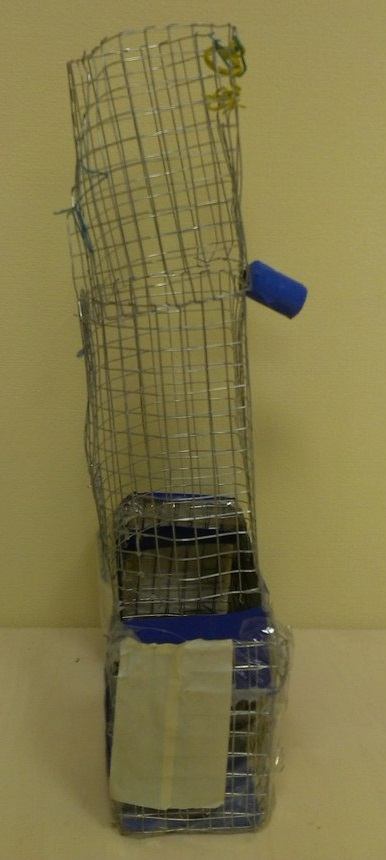
\includegraphics[scale=0.3]{days/18.11.14/images/01}}
	 % 		\caption{Ограничители хода оси}
	 % 	\end{minipage}
	 % \end{figure}

      \item Было замечено, что металлическая сетка, из которой состоит ковш, иногда зацепляется за подъемник, что мешает его движению. Во избежание зацепления, ковш был обклеен скотчем, что позволило сделать его поверхность гладкой.
      
      \item NXT-блок был стационарно закреплен на роботе. Место крепления блока выгодно отличается от первоначального варианта, поскольку во-первых аккумулятор блока теперь легкодоступен, а во-вторых он расположен выше и его труднее повредить в случае столкновения.
      
      \begin{figure}[H]
      	\begin{minipage}[h]{0.2\linewidth}
      		\center  
      	\end{minipage}
      	\begin{minipage}[h]{0.6\linewidth}
      		\center{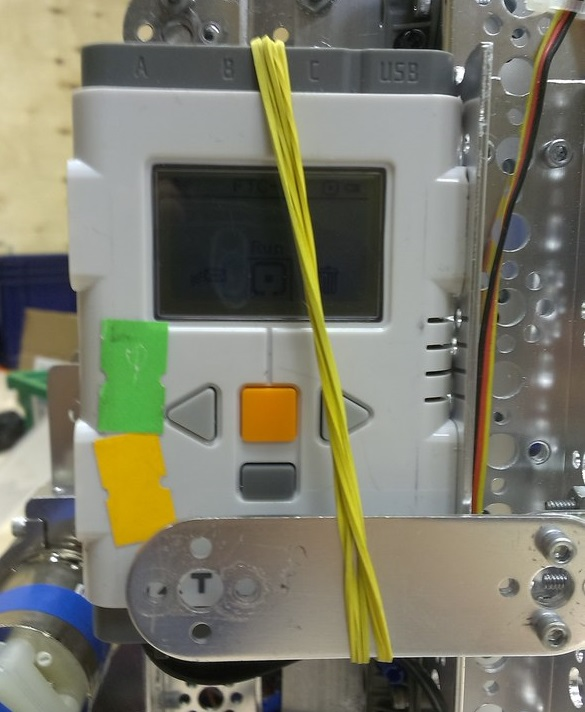
\includegraphics[scale=0.25]{days/19.11.14/images/02}}
      		\caption{Закрепленный NXT-блок (на фото более поздняя версия)}
      	\end{minipage}
      \end{figure}
      
      \item К сожалению, из-за работы над конструкцией робота мы так и не потренировались в управлении им.
          
    \end{enumerate}
    
	\item Итоги собрания: 
	\begin{enumerate}
	  \item Тренировки в управлении роботом не были проведены.
	  	
	  \item NXT-блок закреплен на роботе.
	  
      \item Устранена проблема с зацеплением ковша за подъемник.
      
      \item Ограничители хода оси установлены на подъемник.
      
    \end{enumerate}
    
	\item Задачи для последующих собраний:
	\begin{enumerate}
	  \item Продолжить тренироваться в управлении роботом.
	  
    \end{enumerate}     
\end{enumerate}
\fillpage